% \IUref{IUAdmPS}{Administrar Planta de Selección}
% \IUref{IUModPS}{Modificar Planta de Selección}
% \IUref{IUEliPS}{Eliminar Planta de Selección}

%-------------------------------------- TERMINA descripción del caso de uso.

%\begin{UseCase}[archivo de imágen]{UCX}{Nombre del Caso de uso}{
	\begin{UseCase}{CU8.0}{Eliminar áreas}{
		En esta sección el gerente podrá dar de baja un área que se encuentre registrada, ya sea a 				causa de posibles errores como duplicación de contenido o error a la hora del registro.
	}
		\UCitem{Versión}{1.0}
		\UCitem{Actor}{Gerente}
		\UCitem{Propósito}{Que se agreguen nuevas áreas para realizar alguna actividad.}
		\UCitem{Entradas}{Nombre del área por medio de lista desplegable.}
		\UCitem{Origen}{Los datos serán digitados desde el teclado o bien seleccionados desde una 				lista desplegable.}
		\UCitem{Salidas}{Mensaje de que el área ha sido eliminada exitosamente.}
		\UCitem{Destino}{El área ya no aparecerá en la lista desplegable.
		En la sección consultas el área ya no aparecerá mas.}
		\UCitem{Precondiciones}{Que el área se encuentre registrada previamente.}
		\UCitem{Postcondiciones}{}
		\UCitem{Errores}{Que el sistema no cargue el área para ser eliminada.
		Que el sistema no realice la operación correspondiente }
		\UCitem{Tipo}{Caso de uso primario}
		\UCitem{Observaciones}{}
		\UCitem{Autor}{Francisco García Enríquez.}
		\UCitem{Revisor}{Martin Carrillo.}
	\end{UseCase}

\begin{UCtrayectoria}{Principal}
		\UCpaso[\UCactor] Selecciona del menú principal la opción Áreas.
		\UCpaso Muestra las opciones que el gerente pueda realizar: Registrar Áreas, Consultar Áreas, Eliminar Áreas, Dar de Baja Áreas y Actualizar Áreas.
		\UCpaso[\UCactor] Selecciona la opción eliminar áreas.
		\UCpaso Carga en una lista desplegable las áreas disponible registradas.
		\UCpaso[\UCactor] Selecciona de la lista delegable el área que desea eliminar.
		\UCpaso[\UCactor] Confirma la operación y presiona el botón eliminar.
		\UCpaso Le mostrará un mensaje, {\bf MSG8-}``El dato fue eliminado correctamente''.
		\UCpaso Le muestra una opción para regresar al menú de opciones.
	\end{UCtrayectoria}

\begin{figure}[htbp!]
		\centering
			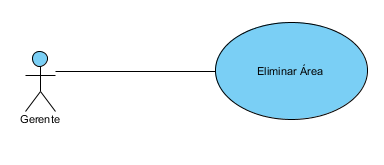
\includegraphics[width=0.8\textwidth]{images/eliminarArea}
		\caption{Diagrama de Casos de Uso del sistema.}
	\end{figure}